\subsection{Satisfiability Modulo Theories Solvers}
In relation to the Satisfiability Solvers, the Satisfiablity Modulo Theories solvers, short SMT solvers, operate on a higher logical level. Because it is often time consuming to formulate your domain specific problem as a boolean formula and transform it into CNF a new class of solvers was defined that try to overcome this restriction. In this section an overview of STP \cite{Ganesh:2007:DPB:1770351.1770421}, which is used in KLEE and other tools, is given.
\todo{maybe add/research something more about first order theories}
In contrast to SAT solvers, STP is able to solve decision problems that contain bit-vectors and arrays. In practice this allows us to reason about various data types such as integers but also certain datastructures like lists and arrays.

As an input STP allows the following operations, which can be grouped in the following way:
\begin{itemize}
\item \textbf{logical and boolean} Constant Values TRUE and FALSE, variables with a boolean value, any boolean operator\footnote{such as $\lor$,$\land$, $\Rightarrow$, etc.}, bitwise boolean operators
\item \textbf{mathematic operations} Left and right shifts, addition, multiplication, unary minus, division, modulo, relational operators
\item \textbf{others} Array read, array write,  extraction of bit-vectors\footnote{$x[i:j]$ is the extraction of the bytes between $i$ and $j$ of $x$ as described in \cite{Ganesh:2007:DPB:1770351.1770421}.}, concatenation of bit-vectors\footnote{The concatenation of two bit-vectors $x_{[n]}$ and $y_{[m]}$ is expressed as $x \circ y$ and returns a new vector $z_{[m+n]}$ of length $m+n$ as described in \cite{Ganesh:2007:DPB:1770351.1770421}.}
\end{itemize}
STP was specifically developed with focus on software analysis projects, because there are often extremely large constraint problems involved. In relation to other SMT solvers STP focuses on reducing the size of a quantifier-free first order logic problem, before it will be converted into conjunctive normal form and solved by a SAT solver\footnote{As a default SAT solver MiniSat\cite{10.1007/978-3-540-24605-3_37} is used.}. This procedure allows it to benefit from the heavily engineered and therefore very fast SAT solvers. Other SMT solvers apply the theory specific decision procedures not until in the included SAT solver, which often leads to problems with the SAT specific optimizations. The architecture of STP is visualized in figure \ref{fig:STP_architecture}.

\todo{add some more content about the "architecture" / flow of STP}
\todo{add more content about the general working of STP, especially the array refinement}

To reduce the size of a problem it applies optimations specific to bit-vector and array theory.
\begin{figure}
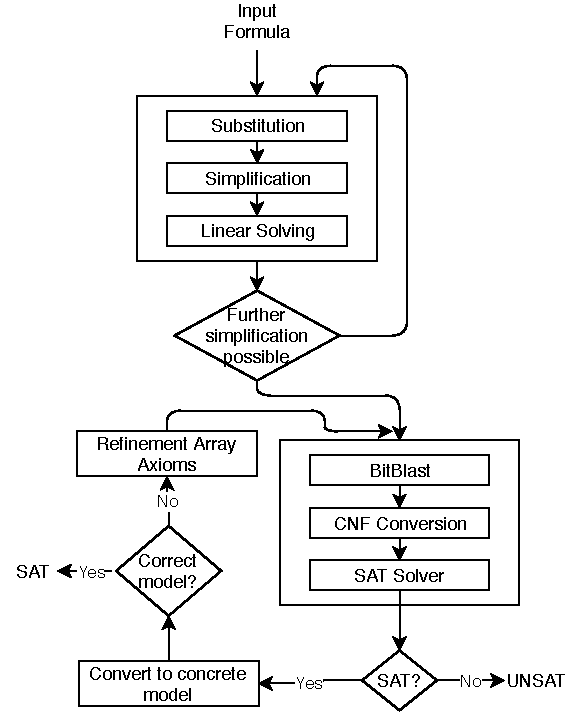
\includegraphics[width=\linewidth]{STP_architecture}
\centering
\caption{STP Architecture}
\label{fig:STP_architecture}
\end{figure}
In the original paper \cite{Ganesh:2007:DPB:1770351.1770421} there are two of these optimizations discussed. The first optimization is an "on-the-fly solver for mod-$2^n$ linear arithmetic" which is embedded in STP. 

When reasoning about fixed length bit-vector arithmetic, this part of the program tries to reason about parts of the bit-vector equation system.
The idea is to use the property of such a vector so that you can always calculate in $\mod{2^b}$ where $b$ is the length of the bit-vector.

There is a mathematical theorem in basic number theory that can be used to determine if a solution to an equation exists if it is$\mod{2^b}$:
$$\sum_{i=1}^{n} a_ix_i = c_i  \Mod{2^b}$$
$$gcd(a_1,...,a_n,2^b) | c_i$$
The equation is only solvable if the greatest common divisor, also known as gcd, is a divisor of every $c_i$.\
Let's assume the following equality system where all variables are bit-vectors with length 3, $b$ is therefore 3:
\todo{replace system with own example}
$$3x+4y+2z=0 \Mod{2^3}$$
$$2x+2y+2=0  \Mod{2^3}$$
$$2x+4y+2z=0 \Mod{2^3}$$
If the $gcd$ of two numbers is $a$ and $m$ is 1, $a$ has per definition a multiplicative inverse in mod $m$. In this particular case $m=2^b$. This property is necessary, because one of the variables needs to be isolated and therefore multiplied with the inverse\footnote{This is neccessary because division in modular arithmetic is defined as the multiplication of the inverse and therefore only works for numbers that have an inverse.}.
The algorithm chooses the first equation and tries to find an $a_i$ where $gcd(a_i,2^3) = 1$ is true.

In the example the algorithm selects $a_1$ which has the value $3$, therefore $x$ can be isolated in the first equation.
The first step is to multiply with the multiplicative inverse of 3 in$\mod{2^3}$ which is also 3.
$$3x+4y+2z = 0 \Mod{2^3} \mid \text{isolate 3x}$$
$$\Leftrightarrow 3x=-4y-2z  \Mod{2^3}  \mid \text{normalize to mod8}$$
$$\Leftrightarrow 3x=4y+6z  \Mod{2^3}  \mid \text{multiple with 3}$$
$$\Leftrightarrow x=12y+18z \Mod{2^3}  \mid \text{normalize to mod8}$$
$$\Leftrightarrow x=4y+2z \Mod{2^3}$$
After $x$ is isolated, it's possible to substitute each $x$ in the original equation system with $4y+2z$ and normalize to$\Mod{2^3}$
$$2(\underbrace{4y+2z}_{x})+2y+2=0 \Mod{2^3} \Leftrightarrow 2y + 4z + 2 = 0\Mod{2^3} $$
$$2(\underbrace{4y+2z}_{x})+ 4y + 2z = 0 \Mod{2^3} \Leftrightarrow 4y + 6z = 0\Mod{2^3} $$
There are no longer any ${a_i}$ in these equations, that have an $gcd(a_i,2^3) = 1$ and therefore no further variable can be isolated.

The algorithm then searches the coefficent $a_i$ which is the smallest in the whole system and chooses the corresponding equation.
After the smallest $a_i$ is choosen the whole system is devided by it and the bit with the highest order is dropped.\todo{maybe rewrite to multiple of bits}

A whole new equation system is formed with linear vectors length $b-1$, in the example two.
The new variables are named $y[1:0]$ and $z[1:0]$ to signal that they represent the bits 1 to 0 of the regarding variable.
$$y[1 : 0] + 2z[1 : 0] + 1 = 0 \Mod{2^2}$$
$$2y[1 : 0] + 3z[1 : 0] = 0\Mod{2^2}$$
Now the first step of isolation a variable $x_i$ with a coefficient $gcd(a_i, 2^b)=1$ is repeated.
$$y[1 : 0] + 2z[1 : 0] + 1 = 0 \Mod{2^2}\mid \text{isolate y[1:0]}$$
$$\Leftrightarrow y[1 : 0] = -2z[1 : 0] -1 \Mod{2^2} \mid \text{normalize to mod4}$$
$$\Leftrightarrow y[1 : 0] = 2z[1 : 0] +3 \Mod{2^2}$$
After isolating $y[1 : 0] $ it's allowed to substitute each $y[1 : 0] $ in the original equation system with $2z[1:0]+3$
$$2(\underbrace{2z[1:0]+3}_{y[1:0]}) + 3z[1 : 0] = 0\Mod{2^2} \mid \text{normalize to mod4}$$
$$\Leftrightarrow 3z[1:0] + 2 = 0 \Mod{2^2}$$
In the last iteration $z[1:0]$ will be isolated because the $gcd(3,2^2) = 1$. The inverse of 3 in$\mod{2^2}$ is 3.
$$3z[1:0] + 2 = 0 \Mod{2^2} \mid \text{isolate 3z[1:0]}$$
$$\Leftrightarrow 3z[1:0]=-2  \Mod{2^2}   \mid \text{normalize to mod4}$$
$$\Leftrightarrow 3z[1:0]=2  \Mod{2^2}   \mid \text{multiple with 3}$$
$$\Leftrightarrow z[1:0]=6  \Mod{4}  \mid \text{normalize to mod4}$$
$$\Leftrightarrow z[1:0]=2  \Mod{4}$$
Because a solution was found it can be concluded that the original equation system is satisfiable.
The original system can be transformed into $$(x = 4y + 6z) \land (y[1 : 0] = 2z[1 : 0] + 3) \land (z[1 : 0] = 2)$$ and forwarded to the SAT solver.
